%% Преамбула TeX-файла

% 1. Стиль и язык
\documentclass[liberation]{G7-32}

% Остальные стандартные настройки убраны в preamble.inc.tex.
\sloppy

% Настройки стиля ГОСТ 7-32
% Для начала определяем, хотим мы или нет, чтобы рисунки и таблицы нумеровались в пределах раздела, или нам нужна сквозная нумерация.
\EqInChapter % формулы будут нумероваться в пределах раздела
\TableInChapter % таблицы будут нумероваться в пределах раздела
\PicInChapter % рисунки будут нумероваться в пределах раздела

% Добавляем гипертекстовое оглавление в PDF
\usepackage[
bookmarks=true, colorlinks=true, unicode=true,
urlcolor=black,linkcolor=black, anchorcolor=black,
citecolor=black, menucolor=black, filecolor=black,
]{hyperref}

\AfterHyperrefFix

\usepackage{microtype}% полезный пакет для микротипографии, увы под xelatex мало чего умеет, но под pdflatex хорошо улучшает читаемость

% Тире могут быть невидимы в Adobe Reader
\ifInvisibleDashes
\MakeDashesBold
\fi

\usepackage{graphicx}   % Пакет для включения рисунков

% С такими оно полями оно работает по-умолчанию:
% \RequirePackage[right=10mm,top=20mm,left=20mm,bottom=20mm,headsep=0pt,includefoot]{geometry}
% Если вас тошнит от поля в 10мм --- увеличивайте до 20-ти, ну и про переплёт не забывайте
\geometry{ignorefoot} % считать от нижней границы текста


% Пакет Tikz
\usepackage{tikz}
\usetikzlibrary{arrows,positioning,shadows}

% Произвольная нумерация списков.
\usepackage{enumerate}

% ячейки в несколько строчек
\usepackage{multirow}

% Для рисования иерархии папок - forest
\usepackage{forest}

\usepackage{fontspec} 


\defaultfontfeatures{Ligatures={TeX},Renderer=Basic}

\setmainfont{Times New Roman}
\newfontfamily\cyrillicfont{Times New Roman}
% \setsansfont{Comic Sans MS}
\setmonofont{Courier New}
\newfontfamily\cyrillicfonttt{Courier New}

% Стиль по умолчанию
\forestset{
  default preamble={
    for tree={
      font=\ttfamily,
      grow'=0,
      child anchor=west,
      parent anchor=south,
      anchor=west,
      calign=first,
      edge path={
        \noexpand\path [draw, \forestoption{edge}]
        (!u.south west) +(7.5pt,0) |- node[fill,inner sep=0pt] {} (.child anchor)\forestoption{edge label};
      },
      before typesetting nodes={
        if n=1
        {insert before={[,phantom]}}
        {}
      },
      fit=band,
      before computing xy={l=15pt},
    }
  }
}

% itemize внутри tabular и выравнивание таблиц
\usepackage{paralist,array,tabularx}

% Немного снимаем боль при работе с таблицами, которые надо центрировать
\newcolumntype{L}{>{\raggedright\arraybackslash}l}
\newcolumntype{P}[1]{>{\raggedright\arraybackslash}p{#1}}
\newcolumntype{M}[1]{>{\centering\arraybackslash}m{#1}}

% tabularx
\newcolumntype{Z}{>{\centering\arraybackslash}X}

%\setlength{\parskip}{1ex plus0.5ex minus0.5ex} % разрыв между абзацами
\setlength{\parskip}{0ex} % разрыв между абзацами
\usepackage{blindtext}

% Центрирование подписей к плавающим окружениям
%\usepackage[justification=centering]{caption}

% Отступ после листинга
\captionsetup[listing]{belowskip=20pt}


% Настройки листингов.
\usepackage{local-minted}

% Полезные макросы листингов.
% Любимые команды
\newcommand{\kt}[1]{\mintinline{kotlin}|#1|}
\newcommand{\codeline}[2]{\mint[style=bw]{#1}|#2|}
\newcommand{\code}[1]{\texttt{#1}}
\newcommand{\todo}[1]{{\color{red}TODO: {#1}}}
\newcommand{\conclusions}{
  \backmatter
  \section{Выводы по разделу}
  \mainmatter
}


% Стиль титульного листа и заголовки


\begin{document}
  % \begin{center}
    \hfill \break
    \footnotesize{\textbf{Министерство науки и высшего образования Российской Федерации}} \\
    \scriptsize{\textbf{ФЕДЕРАЛЬНОЕ ГОСУДАРСТВЕННОЕ АВТОНОМНОЕ ОБРАЗОВАТЕЛЬНОЕ УЧРЕЖДЕНИЕ ВЫСШЕГО ОБРАЗОВАНИЯ}} \\
    \normalsize{\textbf{«НАЦИОНАЛЬНЫЙ ИССЛЕДОВАТЕЛЬСКИЙ \\ УНИВЕРСИТЕТ ИТМО»}} \\
    \hfill \break
    \normalsize{\textbf{ФАКУЛЬТЕТ ЛАЗЕРНОЙ ФОТОНИКИ И ОПТОЭЛЕКТРОНИКИ}} \\
    \hfill \break
    \normalsize{Дисциплина} \\
    \normalsize{<<Полупроводниковые лазеры>>} \\
\end{center}
\hfill \break
\begin{center}
    \large{Реферат} \\
    \normalsize{Генерация оптических частотных гребенок в полупроводниковых лазерах}\\
\end{center}
\hfill \break
\hfill \break
\hfill \break
\begin{flushright}
    Выполнил: \\
    студент группы L3430 \\
    Лапа Н. \\
    Преподаватель: \\
    Ковалёв А. В.
\end{flushright}
\hfill \break
\hfill \break
\hfill \break
\hfill \break
\hfill \break
\begin{center} Санкт-Петербург \\ 2020 \end{center}
\thispagestyle{empty}
\newpage
  % Предварительные приготовления
%   
% Источники, которые будут помещены в верх списка
% \nocite{methodic}

% Переносы слов
% \hyphenation{МИЭТе}


  \frontmatter % выключает нумерацию ВСЕГО; здесь начинаются ненумерованные главы: реферат, введение, глоссарий, сокращения и прочее.

  % \maketitle %создает титульную страницу

  %\listoffigures                         % Список рисунков

  %\listoftables                          % Список таблиц

  %\NormRefs % Нормативные ссылки
  % Команды \breakingbeforechapters и \nonbreakingbeforechapters
  % управляют разрывом страницы перед главами.
  % По-умолчанию страница разрывается.

  % \nobreakingbeforechapters
  % \breakingbeforechapters

  \tableofcontents

  \printnomenclature % Автоматический список сокращений

  \Introduction
\Abbrev{РЧ}{радио частоты}
\Abbrev{VLC (visible light communication)}{связь по видимому свету}

Спустя тридцать лет после появления первых коммерческих мобильных коммуникационных систем, беспроводная связь эволюционировала в обыкновенное удобство как газ или электричество. Экспоненциальный рост в мобильном трафике в течение последних трёх десятилетий привел к масштабному развертыванию беспроводных систем. Как следствие, ограниченный доступный РЧ-диапазон является объектом постоянного переиспользования и межканальной интерференции, что значительно ограничивает ёмкость сетей. Таким образом, было много различных предупреждений о грядущем <<кризисе РЧ спектра>>~\cite{Ofcom2013}, так как требования к передачи мобильных данных данных продолжают расти, в то время как спектральная эффективность сетей насыщается, даже несмотря на введение новых стандартов и значительный технологический прогресс в этой области. По оценкам, к 2022 году более $77$ эксабайтов ($10^{60}$ байт) трафика будет передаваться через мобильные устройства каждый месяц (около одного зеттабайта в год)~\cite{Cisco2019}. В середине прошлого десятилетия было предложено использование связи по видимому свету (VLC) в качестве потенциального решения для избежания <<кризиса РЧ спектра>>.

\Abbrev{ИК}{инфракрасный}
\Abbrev{LED (Light emitting diode)}{светодиод}
\Abbrev{PLC (Power-line communication)}{связь по электросети}
\Abbrev{PoE (Power over Ethernet)}{питание через Ethernet}


В течение прошлого десятилетия значительные усилия были направлены на изучение альтернативных частей электро-магнитного спектра, которые потенциально смогут разгрузить б\'ольшую часть трафика из загруженного РЧ диапазона. Было продемонстрировано использование миллиметровых волн в коммуникации в 28 ГГц диапазоне, а так же использование видимого и ИК света. Это особенно полезно, так как освещение \--- удобство, которое имеется практически в любой жилой среде и для которого существует готовая инфраструктура. Использование видимого света для высокоскоростных линий связи становится возможно из-за использования LED. В этом смысле концепт комбинирования функций освещения и коммуникации позволяет экономить энергию (и деньги) и сократить углеродный след. Во-первых, установка точек доступа является достаточно тривиальной задачей, так как можно переиспользовать уже существующую инфраструктуру с использованием готовых технологий, таких как связь по электросети (PLC) и питание через Ethernet (PoE). Во-вторых, так как освещение обычно работает в помещениях даже в течение светлого времени суток, дополнительное питание передатчиков будет незначительным. Кроме того, открывается возможность использования Li-Fi для Интернета Вещей \--- большого количества умных бытовых устройств, каждому из которых необходимо интернет-соединение для корректной работы. В настоящее время они используют Wi-Fi или проприетарные стандарты связи, что приводит к ещё большей загрузке РЧ-сети и ухудшению совместимости между друг другом. Помимо этого, видимый свет включает в себя сотни ТГц свободного канала, что на четыре порядка больше, чем полный РЧ спектр до 30 ГГц, включая миллиметровый спектр. Оптическое излучение, в общем, не интерферирует с другими радио волнами и не мешает работе чувствительного электрического оборудования. Таким образом, свет идеален для беспроводного покрытия в местах, чувствительных к электро-магнитному излучению (например, больницы, самолёты, топливно-химические и атомные электростанции и другие). Помимо этого, так как свет не может проникать через непрозрачные поверхности (стены), создается более высокий уровень безопасности соединения. Эта же особенность может быть использована для избежания интерференции между двумя соседними сетями.

\Abbrev{RGB (Red-green-blue)}{красный-синий-зелёный}
\Abbrev{MIMO (Multiple-input-mulitple-outputs)}{несколько входов и выходов}
\Abbrev{IM/DD (Intensity modulation and direct detection)}{модуляция интенсивности и прямое детектирования}
\Abbrev{OFDM (Orthogonal frequency division multiplexing)}{мультиплексирование
с ортогональным частотным разделением каналов}
\Abbrev{OWC (Optical wireless communication)}{оптическая беспроводная коммуникация}
\Abbrev{Li-Fi}{light fidelity}
\Abbrev{Wi-Fi}{wireless fidelity}

В течение последних десяти лет, было проведено значительное количество исследований об улучшении скорости передачи между двумя устройствами с использованием существующих светодиодов в лабораторных условиях. В 2012 году была достигнута скорость передачи данных выше 1 Гб/с с использованием белых фосфорных LED~\cite{Khalid2012}, и 3.4 Гб/с с помощью красно-сине-зелёного (RGB) LED~\cite{Cossu2012}. Также была продемонстрирована~\cite{Azhar2013} схожая гигабитная система с белым фосфорным LED в виде матрицы 4 на 4 в конфигурации несколько входов и выходов (MIMO). Теоретическая структура для достижимой ёмкости модуляции интенсивности и прямого детектирования (IM/DD) с использованием мультиплексирования с ортогональным частотным разделением каналов (OFDM) была показана в~\cite{Dimitrov2013}. Для успешной реализации системы мобильной связи необходима готовая сетевая система. Это и есть то, что называется Li-Fi \--- сетевое мобильное высокоскоростное VLC решение для беспроводной связи~\cite{Harald2014}. Гарольд Хаас, которому принадлежит идея создания Li-Fi~\cite{Haas16}, предлагает использовать Li-Fi как комплиментарную сеть для облегчения нагрузки на РЧ спектр, так как значительная часть нагрузки на текущие Wi-Fi сети сможет быть перемещена на Li-Fi сети. 



  \mainmatter % это включает нумерацию глав и секций в документе ниже

  % \chapter{Генерация и применение ЧГ}
\label{ch:research}

\Abbrev{FP}{Fabry-P\'ero \--- Фабри-Перо}
\Abbrev{DFB}{Distributed feedback \--- распределенная обратная связь}
Самым частым способом получения ЧГ является использование лазеров в режиме синхронизации мод, так как для создания ЧГ необходимы фемтосекундные импульсы. Другой метод основан на одном или на каскаде нескольких внешних модуляторов, что требует относительно сложной настройки и в результате получаются высокие потери. Недавно был продемонстрирован простой и дешёвый источник ЧГ, основанный на переключении усиления лазерного диода с внешней инжекцией в Фабри-Перо. Тем не менее, переключение усиления в лазерном диоде с распределённой обратной связью является наиболее простым и надёжным способом генерации импульсов, так что имеет смысл исследовать генерацию ЧГ в DFB лазере~\cite{HuataoZhu2016}. 

В \cite{HuataoZhu2016} было показана экспериментальная установка для генерации ЧГ (рисунок \ref{fig:HuataoZhu}). Он состоит из настраиваемого лазера (TLS), источника радиочастоты и DFB лазера. TLS является главным лазером, и он подсоединен к контроллеру поляризации (PC) для настройки состояния поляризации и к регулируемому оптическому аттенуатору (VOA) для регулировки мощности. Источник радиочастот генерировал синусный сигнал с частотой 10 ГГц, который проходил через усилитель с усилением в 23 дБ, таким образом напрямую модулируя DFB лазер. В конце подключен оптический спектральный анализатор (OSA) для мониторинга оптического спектра.

\begin{figure}[ht]
  \centering
  \includegraphics[width=.8\textwidth]{inc/img/zhu.png}
  \caption{Схематичная диаграмма генератора ЧГ, основанного на инжекционном DFB лазере~\cite{HuataoZhu2016}. Здесь OFCG \--- генератор ЧГ, SG \--- генератор радиочастотного сигнала, Amp \--- усилитель радиочастотного сигнала, DFB \--- распределённая обратная связь, TLS \--- настраиваемый лазерный источник, PC \--- контроллер поляризации, VOA \--- регулируемый оптический аттенуатор, OSA \--- оптический спектральный анализатор.}
  \label{fig:HuataoZhu}
\end{figure}

В результате проведённого эксперимента было установлено, что предложенная конструкция генератора ЧГ может создавать 10 спектральных линий с плоскостью 1.5 дБ. При добавлении в схему фазового модулятора удалось достичь 14 плоских спектральных линий. Предлагаемая схема может быть использована в когерентной оптической коммуникации и микроволновой фотонике.

В \cite{Quirce2018} была исследована поляризационная динамика VCSEL с центральной длиной волны $\lambda=1550$ нм с модуляцией переключения амплитуды усиления для получения ЧГ. Было показано, что благодаря генерации двух перпендикулярных линейно поляризованных гребёнок, результирующая общая ЧГ гораздо шире, чем та, которая была получена из основной поляризации. 

Авторы статьи \cite{Quirce2020} исследовали нелинейную динамику ЧГ, сгенерированных полупроводниковым лазером с оптическими инжекциями. В их эксперименте генератор ЧГ состоял из основного лазера, излучение которого инжектировалось в дополнительный лазер с помощью оптического циркулятора. Количество инжектируемой мощности контролировалось с помощью регулируемого оптического аттенуатора, подключенного к выходу основного лазера, как и в случае выше. Общая схема эксперимента аналогична схеме, представленной на рисунке \ref{fig:HuataoZhu}. Качество полученной ЧГ характеризуется как десяти децибельная спектральная ширина \--- максимальное частотное разделение между пиками со значениями больше 10 дБ ниже, чем абсолютный максимум оптического спектра. 

\begin{figure}[ht]
  \centering
  \includegraphics[width=\textwidth]{inc/img/quirce.png}
  \caption{Оптический спектр полупроводникового лазера с переключением усиления, при токе смещения $I_{bias} = 30$ мА, частота модуляции $f_m = 5$ ГГц, $V_{RF}=0.5$ В, (a) $\Delta v = 6.5$ ГГц и $P_{inj}=417.3$ мкВт, (b) $\Delta v = -0.5$ ГГц и $P_{inj}=330.1$ мкВт, (c) $\Delta v = -1$ ГГц и $P_{inj}=210.5$ мкВт, (d) $\Delta v = -1$ ГГц и $P_{inj}=329.5$ мкВт, (e) $\Delta v = 6.5$ ГГц и $P_{inj}=332.1$ мкВт. Стрелка показывает частоту оптической инжекции~\cite{Quirce2020}.}
  \label{fig:quirce}
\end{figure}

Вообще, для высокоточных лазерных измерений частоты, при которых напрямую измеряется абсолютная оптическая частота, требуются большие газовые лазеры и точечные контактные диоды с коротким периодом жизни, такие как металл-изолятор-металл\--диоды. Кроме того, для системы когерентной оптической коммуникации необходимо измерять разницу частот лазера, которые находятся в диапазоне до нескольких терагерц. Несмотря на это, измерение такой большой разницы частот может вызывать сложности. Относительно недавно был предложен \cite{Kourogi1993} компактный высокоточный измеритель частот на длине волны 1.5 мкм, работа которого основана на генераторе ЧГ. Схема предлагаемого измерителя частот представлена на рисунке~\ref{fig:kourogi}: система состоит из двух частей \--- высокоточного референтного лазерного диода ($LD_R$) на длине волны 1.55 мкм и генератора ЧГ для измерения разницы частот между референтным лазером и измеряемым лазером ($LD_x$), измеряемая разница частот может достигать порядка ТГц.

\begin{figure}[ht]
  \centering
  \includegraphics[width=\textwidth]{inc/img/kourogi.png}
  \caption{Предлагаемая в~\cite{Kourogi1993} система измерения оптической частоты для 1.5 мкм полупроводникового лазера.}
  \label{fig:kourogi}
\end{figure}

Частота референтного лазера фиксирована $\nu_R=(\nu_1 - \nu_2)/2$ при помощи генерации световой волны как суммы и разницы частот референтного лазера и твердотельного лазера на длине волны 1.06 мкм ($\nu_S$), и с помощью фиксирования суммы и разницы частот на частотах ($\nu_1$ и $\nu_2$) двух стабилизированных He-Ne лазеров, где $\nu_1$ и $\nu_2$ \--- абсолютные частоты этих лазеров. Можно использовать LiNbO3 для сложения и вычитания частот. Так как гетеродинное измерение очень чувствительное, не требуется высокая мощность сигналов.

Генератор ЧГ генерирует модуляционные боковые полосы из падающего лазерного излучения, и эти боковые полосы используются как локальные осцилляторы для измерения разницы частот между референтным лазером и измеряемым лазером. Точность измерения разницы частот может быть равна частоте модуляции. Для высокой точности измерения необходим ``широкий'' генератор ЧГ. На рисунке~\ref{fig:kourogi2} представлена его конструкция. Он состоит из электро-оптического фазового модулятора, установленного в резонатор Фабри-Перо. Модулятор является покрытым антибликовым покрытием кристаллом LiNbO3, установленным в микроволновый волновод. Для того, чтобы он был высокоэффективным для высоких частот, ширина волновода была выбрана для резонанса микроволн, чтобы концентрировать микроволны в кристалле. 

\begin{figure}[ht]
  \centering
  \includegraphics[width=\textwidth]{inc/img/kourogi2.png}
  \caption{Конструкция генератора ЧГ, использованного в в~\cite{Kourogi1993}.}
  \label{fig:kourogi2}
\end{figure}

\Abbrev{WDM}{Wavelength division multiplexed \--- мультиплексирование с разделением по длине волны}
\Abbrev{OTDM}{Optical time division multiplexed \--- мультиплекирование с разделением по оптическму времени}
\Abbrev{MLL}{Modelocked laser \--- лазер в режиме синхронизации мод}
В статье \cite{Delfyett2006} авторы показывают потенциал применения ЧГ в коммуникациях с ультравысокой пропускной способностью и процессинге сигналов как показано на рисунке \ref{fig:delfyett}. Этот рисунок показывает как оптические ЧГ могут быть использованы в:

\begin{enumerate}
  \item Аналоговом и цифровом WDM формате, когда каждая из полос гребёнки модулируется независимо и когерентно детектируется при помощи гребёнок отдельного синхронизированного приёмного MLL;
  \item Ультравысоко скоростные форматы OTDM, при которых высокоскоростные последовательности импульсов демультиплексируются по времени с помощью синхронизированного приёмника MLL;
  \item Мультиплексирование с разделением по оптическому коду, при котором переданные импульсы модулируются при помощи включения\--выключения и закодированы спектральной фазой, а приём осуществляется когерентным гомодинным детектором при помощи синхронизированного приёмника MLL.
\end{enumerate}

\begin{figure}[ht]
  \centering
  \includegraphics[width=\textwidth]{inc/img/delfyett.png}
  \caption{Использование ЧГ для модуляции в временной области, частотной области и кодовой области~\cite{Delfyett2006}.}
  \label{fig:delfyett}
\end{figure}

В итоге авторы показали, что частотные гребёнки полученные при помощи MLL являются идеальными оптическими синусоидами для большого количества различных применений в когерентной обработке сигналов, особенно для генерации произвольных длин волн и для архитектуры когерентного приёмника. Ключевой потребностью при таком применении является стабильность и надёжность генератора оптических ЧГ. 

\Abbrev{MZ}{Mach-Zender \--- [модулятор/интерферометр] Маха-Цендера}
В другой статье \cite{Yokota2015} авторы исследуют ЧГ, сгенерированную InP полупроводниковым MZ-модулятором с помощью численной модели, которая принимает во внимание нелинейность изменения коэффициента преломления и оптическое поглощение, вызванное напряжением, приложенным к модулятору. Эта нелинейность крайне мала для обычных MZ-модуляторов на основе LiNbO3, но становятся заметными для полупроводниковых MZ-модуляторов. 

Роутинг на основе WDM является незаменимой технологией для сетевых фотонных систем следующего поколения, в которых длина волны определяет пункт назначения сигнала. Такая система требует многоканальный оптический передатчик, который можно получить при комбинации WDM-модулятора и генератора ЧГ. В этой работе исследователи описывают девяти-канальную ЧГ, сгенерированную InP-MZ модулятором с помощью численных методов. Схематичное изображение экспериментальной установки и ЧГ приведено на рисунке \ref{fig:yokota}

\begin{figure}[ht]
  \centering
  \includegraphics[width=\textwidth]{inc/img/yokota.png}
  \caption{(a) Схема экспериментальной установки и (b) ЧГ~\cite{Yokota2015}.}
  \label{fig:yokota}
\end{figure}

В другой статье \cite{Yokota_2015} эти же авторы численную модель модулятора Маха-Цендера, который показан на рисунке \ref{fig:yokota}: постоянное напряжение $V_{DC1}$ и $V_{DC2}$ был приложен к плечам №1 и №2 соответственно. Помимо него к обоим плечам было приложено переменное напряжение $V_{AC}$ в виде синусоидального радиочастотного напряжения. Напряжение на первом плече было меньше, чем на втором. Тогда напряжения $V_1$ и $V_2$ можно записать следующим образом:

\begin{equation}
  V_1 = aV_{AC}\sin(\omega_m t) + V_{DC1}
\end{equation}

\begin{equation}
  V_2 = -V_{AC}\sin(\omega_m t) + V_{DC2}
\end{equation}

где $\omega_m$ \--- угловая частота переменного тока. Когда $V_1$ и $V_2$ приложены модулятору, выходное электрическое поля модулятора $E_o$ записывается следующим образом:

\begin{equation}
  E_o = \frac{E_i}{2} \left[ c_1(V_1)e^{j\{\omega t - \phi_1(V_1) - \Delta \phi\}} + c_2(V_2) e^{j\{\omega t-\pi_2(V_2)\}} \right]
\end{equation}

где $\phi_1$ и $\phi_2$ \--- изменения фазы, а $c_1$ и $c_2$ \--- коэффициенты, определяемые оптическим поглощением в каждом плече. 

\begin{figure}[ht]
  \centering
  \includegraphics[width=\textwidth]{inc/img/yokota2.png}
  \caption{(a) Девиация интенсивности девятиканальной ЧГ и (b) соответствующее напряжение по отношению к переменному напряжению. Кругами, треугольниками и квадратами обозначены измеренные значения. Сплошными, пунктирными и точечными линиями обозначены вычисленные значения~\cite{Yokota_2015}.}
  \label{fig:yokota2}
\end{figure}

При сравнении измеренных значений с вычисленными по модели (см. рис. \ref{fig:yokota2}) хорошо видно, что модель хорошо описывает экспериментальные измерения. Важно отметить, что это значения не совпадают только в случае, когда принимается во внимание линейная часть изменения показателя преломления в модуляторе. Эта модель показывает, что нельзя пренебрегать нелинейностью показателя преломления и оптическим поглощением в полупроводниках при оценки плоскости ЧГ.

Важно также отметить и применение ЧГ в спектроскопии, так как с помощью них можно значительно улучшить существующие интерферометры Майкельсона с Фурье преобразованием. Создаётся новый класс инструментов \--- спектрометры с двойной гребёнкой, в них нет движущихся частей, что позволяет получить более быстрые и точные измерения для больших спектральных интервалов~\cite{Picqu2019}.

В большинстве случаев, генератор ЧГ является широкополосным источником света, который одновременно возбуждает несколько (много) переходов в исследуемом образце. Тогда необходим спектрометр (за исключением случаев с маленькой шириной ЧГ или с очень простым спектром). Если спектрометр имеет достаточное разрешение, можно рассматривать отдельные линии ЧГ, что позволяется использовать само-калибровку по частоте. Тогда разрешение определяется как частота повторения гребёнки $f_{rep}$, несмотря на то, что спектральные элементы могут быть определены со значительно более высокой точностью. Когда разрешение спектрометра равно (или лучше) расстоянию между линиями в гребёнке, инструментальная форма линии начинает определяться шириной линий гребёнки, а не откликом спектрометра. Когда ширина линий гребёнки становится \'уже, вклад инструментальной формы линии становится пренебрежимо малым, так как атомные или молекулярные резонансы имеют ширину равную (или большую), чем расстояние между линиями в гребёнке $f_{rep}$. 

Виды спектроскопических техник с использованием ЧГ (все техники представлены на рисунке~\ref{fig:picqu}):

\begin{itemize}
  \item прямая ЧГ спектроскопия \--- (рис.~\ref{fig:picqu}a) является самым простым подходом к линейной или нелинейной ЧГ спектроскопии. Для линейной спектроскопии одна линия гребёнки резонирует с переходом, а все остальные линии, в идеале, не должны совпадать с резонансами. Для двух-фотонной спектроскопии, много пар линий ЧГ с одинаковой суммой частот делают вклад в возбуждение, что является настолько же эффективным, как и возбуждение непрерывным лазерным пучком с такой же средней мощностью; 
  \item спектроскопия Рамзи гребёнок \--- (рис.~\ref{fig:picqu}b) измеряет интерференцию между возбуждениями атомных или молекулярных образцов с помощью двух интенсивных задержанных во времени импульсов, выведенных из ЧГ;
  \item спектроскопия с использованием дисперсионного спектрометра \--- (рис.~\ref{fig:picqu}c) является простым и надёжным инструментом для мультиканальной параллельной широкополосной спектроскопии с ЧГ. Было успешно продемонстрировано использование решёток со сканирующими детекторами или камерами;
  \item основанная на интерферометре Майкельсона Фурье спектроскопия \--- (рис.~\ref{fig:picqu}d) является наиболее успешной техникой спектроскопии на протяжении уже более 50 лет. Обычно используется некогерентный источник света, а спектрометр измеряет интерференцию двух сигналов из двух плеч с разным оптическим ходом. При использовании ЧГ в качестве источника света, частота каждой линии сдвигается при отражении в движущимся плече интерферометра на $-2(nf_{rep}+f_0)v/c$. Когерентный источник излучения, такой как генератор ЧГ, имеет более высокую яркость, что приводит к возрастанию отношения сигнала к шуму и снижению времени измерения;
  \item двух гребёночная спектроскопия \--- (рис.~\ref{fig:picqu}e) новый подход к Фурье спектроскопии без движущихся частей. В большинстве реализаций ЧГ с частотой повторения $f_{rep}$ после прохождения через образец сталкивается со второй гребёнкой с чуть другой частотой повторения $f_{rep}+\delta f_{rep}$, которая работает как локальный осциллятор. Интерференционный сигнал записывается как функция от времени, после чего производится Фурье преобразование для получения спектра. Фундаментальное отличие между двух гребёночными спектрометрами и традиционными заключается в свободе геометрии. С рассеивающим или интерференционным инструментом теоретическая разрешающая способность может быть записана как $R = \Delta/\lambda$, где $\Delta$ \--- максимальная разность оптического пути, а $\lambda$ \--- длина волны. С двух гребёночным интерферометром разрешающая способность записывается иначе: $R = T/\tau$, где $T$ \--- время измерения, а $\tau$ \--- период световой вибрации. Таким образом, двух гребёночная спектроскопия является единственной техникой, которая потенциально может достичь разрешения равного интервалу между линиями гребёнки, что позволяет открыть новые возможности для прецизионной спектроскопии и метрологии. 
\end{itemize}

\begin{figure}[ht]
  \centering
  \includegraphics[width=.6\textwidth]{inc/img/picqu.png}
  \caption{Методы спектроскопии с использованием ЧГ: (а) прямая ЧГ спектроскопия, (b) спектроскопия Рамзи гребёнок, (с) спектроскопия с использованием дисперсионного спектрометра, (d) основанная на интерферометре Майкельсона Фурье спектроскопия, (e) двух гребёночная спектроскопия~\cite{Picqu2019}.}
  \label{fig:picqu}
\end{figure}

  \chapter{Обзор системы VLC}

\section{Li-Fi и VLC}

\Abbrev{IM}{intensity modulation}
\Abbrev{DD}{direct detection}
\Abbrev{IEEE (Institute of Electrical and Electronics Engineers)}{институт электроники и инжинеров электроники}

В VLC данные передаются при помощи модуляции интенсивности излучения источника (светодиода) \--- IM. Приёмником в такой системе может выступать фотодетектор, который использует принцип прямого детектирования (DD). VLC был придуман для связи <<от точки к точке>>, то есть как замена кабелям~\cite{Haas16}. Работа VLC описывается стандартом IEEE 802.15.7-2018~\cite{IEEE2018}.

С другой стороны, Li-Fi описывает полную беспроводную сеть с возможностью двусторонней коммуникации <<от точки к многим точкам>> и  <<от многих точек к точке>>. Помимо этого, Li-Fi включает в себя возможность использования многих точек доступа с быстрым переключением между ними, что позволяет обеспечить мобильность пользователей. То есть стандарт Li-Fi включает в себя стандарт VLC, что показано на схеме \ref{fig:vlcvslifi}.

\begin{figure}[!ht]
    \centering
    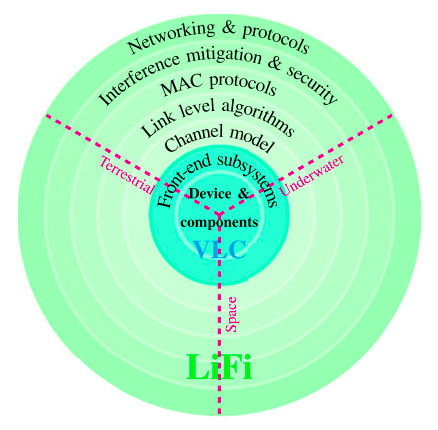
\includegraphics[width=.6\textwidth]{inc/img/vlcvslifi.png}
    \caption{Принципиальная схема Li-Fi и VLC~\cite{Haas16}}
    \label{fig:vlcvslifi}
\end{figure}

Как и было описано во введении, Li-Fi имеет ряд преимуществ по сравнению с Wi-Fi: он позволяет обеспечить безопасность передачи данных, отсутствие интерференции с ЭМ-приборами, разгрузка РЧ-спектра.

\section{Li-Fi передатчик}

Зачастую в системах передачи информации с помощью видимого света в качестве передатчика выбирается светодиодный светильник (LED luminaire)~\cite{LeMinh2008,Komine2006,Komine2004}. Он представляет из себя полноценное осветительное устройство, состоящее из LED источник излучения, балласта, корпуса и других компонентов. LED источник может состоять из одного или нескольких светодиодов, которые управляются с помощью управляющей микросхемы \--- контроллера, который контролирует ток, питающий светодиод и меняющий его яркость. Когда светодиодный светильник используется для коммуникации, контроллер модернизируется для передачи данных с помощью модуляции излучения. Примером простейшей модуляции является On-Off Keying, то есть <<нули>> и <<единицы>> передаются как два разных уровня интенсивности света.

Ключевым требованием к конструкции системы Li-Fi является то, что освещение, которое является основной целью светодиодных светильников, не должно нарушаться из-за использования связи. Таким образом, на работу Li-Fi системы влияет конструкция светодиодного светильника. Белый свет является самым используемым для освещения в помещениях и на улице. Это связано с тем, что цвет предметов под белым светом наиболее сильно похож на цвет предметов под естественным светом. Белый свет у LED светильников достигается двумя разными способами: 

\begin{enumerate}
    \item Синий LED с фосфором \--- этот источник генерирует белый свет с использованием синего LED, который покрыт жёлтым фосфором. Когда синий свет проходит через жёлтое покрытие, эта комбинация создаёт белый свет. При изменении толщины покрытия можно получать белый свет различной цветовой температуры.
    \item Комбинация RGB светодиодов \--- белый свет может быть получен при смешении красного, зелёного и синего света. Для этого, соответственно, необходимо три светодиода, что повышает стоимость светильника, по сравнению с синим фосфорным LED. 
\end{enumerate}

В осветительных системах чаще всего используется первый тип светодиодов из-за их дешевизны, однако в коммуникационных системах фосфорное покрытие значительно ограничивает скорость, с которой светодиод можно переключать, до нескольких МГц~\cite{Khalid2012}. С другой стороны, использование нескольких цветных светодиодов позволяет использовать Color Shift Keying модуляцию при помощи трёх длин волн, что позволяет получить высокую скорость передачи данных и низкую стоимость LED~\cite{Bian2019}.

\section{Li-Fi приёмник}

В качестве приёмников в Li-Fi системах чаще всего используются

\begin{enumerate}
    \item фотодетекторы \--- фотодиоды,
    \item датчики изображения \--- камеры.
\end{enumerate}

Фотодетектор \--- полупроводниковое устройство, которое генерирует ток при падении на него света. Современные коммерческие фотодетекторы могут детектировать с частотой до десятков МГц. 

\Abbrev{FPS (frames per second)}{кадры в секунду}
\Abbrev{IoT (internet of thing)}{интернет вещей}

Помимо него, возможно и использование камеры, так как они уже встроены в большинство потребительской техники (смартфоны, ноутбуки), что позволяет сделать эти устройства приёмниками в Li-Fi системе. Помимо этого, открывается возможность использования Li-Fi для интернета вещей (IoT)~\cite{Duquel2018}. По сути, камера является матрицей фотодетекторов на плате. Существенным недостатком является то, что так как камеры приспособлены для получения изображений высокого разрешения, используется большое количество фотодетекторов, что значительно снижает количество кадров в секунду (FPS) \--- скорость обработки излучения. Например, камеры современного смартфона позволяют записывать видео с 60 FPS, что означает, что использование камеры значительно ограничивает скорость получения информации. 

Важно отметить, что несмотря на то, что использование камеры позволяет превратить любое мобильное устройство в приёмник, пропускная способность остаётся очень ограничена (порядка килобит в секунду). В то же время отдельные фотодетекторы позволяют принимать информацию с высокой пропускной способностью (сотни мегабит в секунду).

\section{Методы модулирования излучения}

% http://www.phpathak.com/files/vlc-comsoccst.pdf p 10

Самое важное отличие системы связи по видимому свету от РЧ-связи заключается в том, что в VLC информация не может быть закодирована в амплитуде и фазе света~\cite{Tsonev2013}. Это означает, что техники модуляции, использующие модулирование фазы и амплитуды не могут быть применены в VLC, и информация должна быть закодирована в интенсивности света \--- модуляция интенсивности (IM). При создании Li-Fi системы необходимо учитывать параметры освещения, некоторые из которых могут повлиять на человека. Пример таких параметров: 
% Существуют различные техники модуляции интенсивности, некоторые из них будут рассмотрены ниже.

\begin{enumerate}
    \item затемнение\footnote{dimming}. В~\cite{Zukauskas2002} было показано, что для разных действий необходимы разные уровни яркости освещения. Например, освещение в интервале $30-100$ лк обычно является достаточным для освещения общественных мест. С другой стороны, для освещения офисов и домов необходима освещённость порядка $300-1000$ лк. Благодаря развитию технологии светодиодных драйверов, становится возможно затемнять светодиоды до любого необходимого уровня в зависимости от применения и требований по сохранению энергии;
    \item смягчение мерцания\footnote{flicker mitigation}. Для системы коммуникации по видимому свету необходимо, чтобы человек не замечал мерцание яркости света. В~\cite{Berman1991} было показано, что мерцание может вызывать серьезные физиологические последствия у людей. Поэтому, необходимо модулировать свет с более высокой частотой, чем частота, которую может воспринимать человеческий глаз. В стандарте IEEE 802.15.7~\cite{IEEE2018} предложено использовать модуляцию интенсивности с частотой выше 200 Гц для избежания вреда для здоровья. 
\end{enumerate}

Рассмотрим четыре типа модуляции, которые применяются в VLC: 

\Abbrev{ИМ}{импульсная модуляция}
\Abbrev{CSM (color shift modulation)}{цветовая манипуляция}

\begin{enumerate}
    \item On-Off Keying (OOK);
    \item импульсная модуляция (ИМ);
    \item мультиплексирование с ортогональным частотным разделением каналов;
    \item цветовая манипуляция (CSM);
\end{enumerate}

\subsection{On-Off Keying}

\Abbrev{NRZ}{non-return-to-zero [on-off-keying]}

В OOK биты данных 1 и 0 передаются включением и выключением светодиода соответственно. В выключенном состоянии светодиод не выключен до конца, но интенсивность его излучения уменьшена. К преимуществам OOK относят простоту реализации. Схожая модуляция используется в волоконных коммуникациях. Большинство ранних работ с использованием OOK в VLC использовали белый светодиод. Если используется синий светодиод с фосфором, то его пропускная способность сильно ограничена (в связи с временем релаксации \--- несколько МГц~\cite{Grubor2007}). Было предложено~\cite{Park2007} использовать <<не возвращающийся к нулю>>\footnote{non-return-to-zero (NRZ)} OOK с синим светодиодом, то можно достичь пропускной способности порядка десятков Мб/с. Помимо этого, можно использовать~\cite{Grubor2007} синий фильтр, чтобы из сигнала медленно реагирующий жёлтый фосфор, в результате чего повысив скорость передачи данных до 40 Мб/c. Аналогично в~\cite{Minh2008,Vucic2009} было предложено комбинирование синего фильтра и аналогового выравнивания на приёмнике для достижения скорости передачи данных 100 и 125 Мб/с соответственно. В~\cite{Vucic2010} было показано, что производительность можно увеличить при помощи лавинных фотодиодов (а не p-i-n фотодиод) в качестве приёмника. Достижимая скорость передачи данных с лавинным фотодиодом и NRZ-OOK составила около 230 Мб/с~\cite{Vucic2010}. В~\cite{Fujimoto2013} использовался RGB светодиод (который лишен основного недостатка фосфорных светодиодов \--- ограничения частоты модуляции из-за времени релаксации). Однако в этой работе модуляция происходила только по одному цветовому каналу \--- красному, в то время как остальные были использованы для создания постоянного белого освещения. Полученная система достигла скорости передачи данных 477 Мб/с с простой NRZ-OOK модуляцией и p-i-n фотодиодным приёмником. 

\subsection{Методы импульсной модуляции}

\Abbrev{PWM (pulse width modulation)}{модуляция длительности импульса}
\Abbrev{PPM (pulse position modulation)}{фазово-амплитудная модуляция}

Несмотря на то, что OOK имеет ряд преимуществ (простота и лёгкость реализации), оно имеет значительное ограничение \--- низкая скорость передачи данных. Поэтому были разработаны альтернативные методы модуляции, которые основаны на длительности (PWM) и положении импульса (PPM). 


\subsubsection{Модуляция длительности импульса}

PWM является эффективным способом модуляции при помощи затемнения. При PWM длительность импульсов выбирается исходя из желаемого уровня затемнения, в то время как сами импульсы несут модулированный сигнал. Этот сигнал передается в импульсе, во время которого светодиод работает на полной мощности. В~\cite{Sugiyama2007} было показано, что затемнение от $0\%$ до $100\%$ может быть получено с высокой частотой PWM. Одним из преимуществ PWM является возможность достижения затемнения без изменения интенсивности импульсов, что не приводит к изменению цвета (что может происходить в OOK). К ограничениям PWM можно отнести ограниченную скорость передачи данных (4.8 Кб/с в~\cite{Sugiyama2007}). 

\subsubsection{Фазово-амплитудная модуляция}

PPM является другим способом импульсной модуляции, основанным на фазе импульса. При PPM длина символа информации разделена на на $t$ слотов одинаковой длительности, а импульс помещается в один из таких слотов. Положение импульса определяет переданный символ. Из-за этой простоты многие ранние разработки (\cite{Georghiades1994,Shiu1999}) оптических беспроводных систем связи использовали именно этот тип модуляции. В~\cite{Gfeller1996} авторы предлагают использование системы с адаптивной частотой передачи и повторением сигналов, что позволяет улучшить передачу данных в условиях плохого соединения. 

\Abbrev{OPPM (overlapping pulse position modulation)}{перекрывающаяся фазово-амплитудная модуляция}

Из-за ограничений, вызванных низкой спектральной эффективностью и скоростью передачи данных при помощи PPM (только один импульс за длительность символа $t$), были предложены другие варианты фазово-амплитудных модуляций. Обобщенно они называются перекрывающимися фазово-амплитудными модуляциями (OPPM), в которых возможна передача более чем одного импульса за время длительности символа~\cite{Shiu1999} и перекрывание нескольких символов (см. рисунок~\ref{fig:ppmvspwm}). В~\cite{BoBai2010} было показано, что OPPM не только позволяет достичь более высокой спектральной эффективности по сравнению с PPM и OOK, но и предоставляет более широкий интервал уровней затемнения, которые могут быть получены, наряду с более высокими скоростями.  

\begin{figure}[!ht]
    \centering
    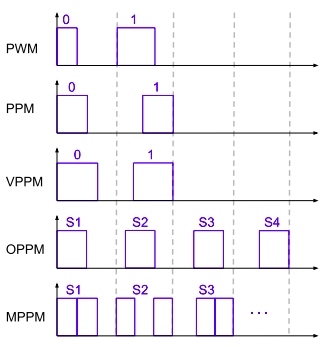
\includegraphics[width=.5\textwidth]{inc/img/ppmvspwm.png}
    \caption{Схематическая диаграмма, показывающая различия между модуляцией длительности импульса (PWM), фазово-амплитудной модуляцией (PPM), переменной фазово-амплитудной модуляцией (VPPM), перекрывающейся фазово-амплитудной модуляцией (OPPM) и многоимпульсной фазово-амплитудной модуляцией (MPPM). $S_n$ обозначает n-ный символ.~\cite{Pathak2015}}
    \label{fig:ppmvspwm}
\end{figure}

\Abbrev{MPPM (multipulse pulse position modulation)}{многоимпульсная фазово-амплитудная модуляция}
Другим обобщением PPM (предложено в~\cite{Sugiyama1989}) является схема, называемая многоимпульсная фазово-амплитудной модуляцией (MPPM). Как и в OPPM, она позволяет передавать несколько импульсов за время длительности одного символа, однако MPPM отличается от OPPM тем, что в первой импульс не должен быть непрерывным (см. рис.~\ref{fig:ppmvspwm}). В~\cite{Shiu1999} было показано, что MPPM может достичь более высокой спектральной эффективности, по сравнению с OPPM.

\Abbrev{VPPM (variable pulse position modulation)}{переменная фазово-амплитудная модуляция}

Стандарт IEEE 802.15.7~\cite{IEEE2018} предлагает схему модуляции, которая называется переменная фазово-амплитудная модуляция (VPPM) и является гибридом PPM и PWM. В VPPM биты закодированы фазой импульса, как и в PPM, но длительность импульса может быть изменена в зависимости от требований (см. рисунок~\ref{fig:ppmvspwm}). VPPM обладает простотой и надежностью PPM и позволяет иметь большее количество уровней затемнения за счёт разной длительности импульсов.

\subsubsection{Мультиплексирование с орто­гональным частотным разделением каналов (OFDM)}

Одним из ограничений модуляций описанных выше является то, что они подвержены межсимвольной интерференции из-за нелинейного частотного отклика каналов связи, основанных на видимом свете. OFDM широко используется в РЧ-связи, так как она позволяет избежать межсимвольную интерференцию. В~\cite{Afgani2006} авторы впервые предложили использование OFDM для VLC. В OFDM канал разделён на несколько ортогональных несущих, по которым данные отправляются параллельными потоками, модулируемыми по несущим. Проблема применения OFDM для беспроводных систем связи по видимому свету заключается в том, что OFDM генерирует комплексные биполярные сигналы, которые необходимо сконвертировать в действительные сигналы.

Другой проблемой OFDM является нелинейность отношения приложенного тока к интенсивности света LED~\cite{Burchardt2014}. Это выражается в отношении пиковой к средней мощности и было изучено в~\cite{Elgala2009,Elgala2009}. Там авторы предлагают в качестве решения использование светодиода в небольшом интервале, на котором это отношение квазилинейное. 

Несмотря на эти недостатки, OFDM  имеет высокие перспективы, и было показано, что возможно достижение скорости передачи до нескольких Гб/с с использованием одного светодиода~\cite{Khalid2012,Tsonev2014}.

\subsubsection{Цветовая манипуляция (CSK)}

В стандарте IEEE 802.15.7~\cite{IEEE2018} описывается ещё один тип модуляции, который был разработан специально для использования в беспроводных системах связи по видимому свету \--- цветовая манипуляция (CSK). Суть этого метода заключается в отдельном модулировании трёх цветовых компонент RGB светодиода. 

\begin{figure}[!ht]
    \centering
    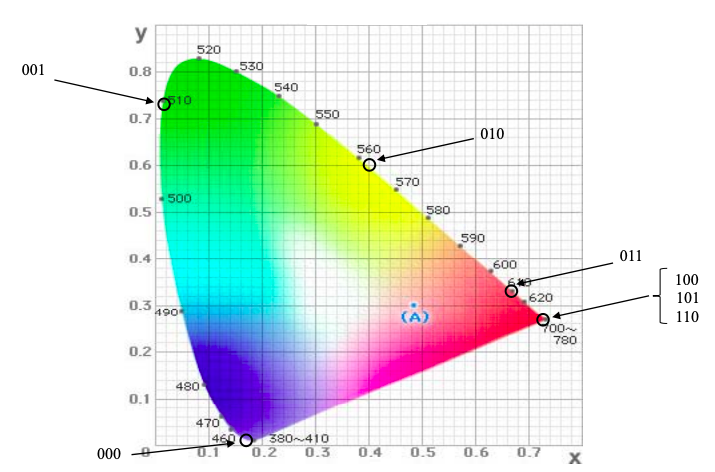
\includegraphics[width=.65\textwidth]{inc/img/cie1931.png}
    \caption{Цветовое пространство CIE 1931~\cite{IEEE2018}}
    \label{fig:cie1931}
\end{figure}

CSK модуляция основана на модели цветового пространства CIE 1931~\cite{CIE1931} (рисунок~\ref{fig:cie1931}, таблица~\ref{table:cie1931}), на которой всем видимым человеческим глазом цветам присвоена пара $(x,y)$ координат. Все это пространство разделено на семь полос, представленных в таблице~\ref{table:cie1931}

\begin{table}[!h]
    \centering
    \begin{tabular}{|c| c| c| c|} 
     \hline
     Полоса (нм) & Код & Центральная длина волны (нм) & $(x,y)$ \\ \hline
     $380-478$ & $(000)$ & $429$ & $(0.169, 0.007)$ \\ \hline
     $478-540$ & $(001)$ & $509$ & $(0.011, 0.733)$ \\ \hline
     $540-588$ & $(010)$ & $564$ & $(0.402, 0.597)$ \\ \hline
     $588-633$ & $(011)$ & $611$ & $(0.669, 0.331)$ \\ \hline
     $633-679$ & $(100)$ & $656$ & $(0.729, 0.271)$ \\ \hline
     $679-726$ & $(101)$ & $703$ & $(0.734, 0.265)$ \\ \hline
     $726-780$ & $(110)$ & $754$ & $(0.734, 0.265)$ \\ \hline
    \end{tabular}
    \caption{Семь полос, используемых в CSK, их коды, центральные длины волн и координаты на цветовом пространстве~\cite{IEEE2018}}
    \label{table:cie1931}
\end{table}

Суть алгоритма кодирования информации заключается в следующем~\cite{IEEE2018}:

\begin{enumerate}
    \item выбираются три точки в цветовом пространстве, которые соответствуют цветам RGB светодиода \--- получается треугольник;
    \item в зависимости от выбранной схемы кодирования (4-CSK, 8-CSK, 16-CSK \--- четыре, восемь и шестнадцать символов, соответственно) определяются координаты символов на плоскости. По сути это является задачей на оптимизацию, так как необходимо выбрать координаты так, чтобы расстояние между ними было наибольшим (это необходимо для минимизации интерференции между символами);
    \item по координатам символов вычисляется яркость компонент RGB светодиода:
    \begin{equation}
        \begin{gathered}
            x_s = P_i x_i + P_j x_j + P_k x_k \\
            y_s = P_i y_i + P_j y_j + P_k y_k \\
            P_i + P_j + P_k = 1
        \end{gathered}
    \end{equation}

    Здесь $(P_i, P_j, P_k)$ \--- яркости компонент светодиода, $(x_s, y_s)$ \--- цветовые координаты символа на цветовой плоскости (рисунок~\ref{fig:cie1931}), $(x_{ijk}, y_{ijk})$ \--- координаты центральных длин волн компонент светодиода на цветовой плоскости. 
\end{enumerate}


  \chapter{Методы модулирования излучения}

В VLC системах информация кодируется при помощи модуляции фазы, амплитуды и интенсивности. При рассмотрении различных схем модуляции необходимо не забывать об использовании системы в качестве освещения, так как некоторые параметры могут влиять на психо-физическое состояние человека. Некоторые такие параметры:

\begin{enumerate}
    \item затемнение \--- для разных сценариев освещения необходимы различные уровни освещенности~\cite{Zukauskas2002}. Если для освещения общественных пространств обычно достаточно света в интервале $30-100$ лк, то для освещения офисов и жилых помещений нужно освещение $300-1000$ лк. Современные светодиодные драйверы, управляющие питанием светодиодов, позволяют устанавливать любые необходимые уровни освещения в зависимости от сценария использования и требований по экономии энергии;
    \item смягчение мерцания \--- так как модуляция интенсивности подразумевает высокочастотное изменение интенсивности источника света, необходимо выбирать такой интервал частот, который не воспринимается человеческим глазом. Было показано (\cite{Berman1991}), что заметное мерцание освещения в течение продолжительного периода времени может привести к физиологическим последствиям у людей. Основной стандарт, описывающий системы VLC и Li-Fi \--- IEEE 802.15.7~\cite{IEEE2018} \--- рекомендует использовать частоту модулирования интенсивности не ниже 200 Гц.
\end{enumerate}

Рассмотрим четыре типа модуляции, которые применяются в VLC: 

\Abbrev{ИМ}{импульсная модуляция}
\Abbrev{CSM (color shift modulation)}{цветовая манипуляция}

\begin{enumerate}
    \item On-Off Keying (OOK);
    \item импульсная модуляция (ИМ);
    \item мультиплексирование с ортогональным частотным разделением каналов;
    \item цветовая манипуляция (CSM);
\end{enumerate}

\section{On-Off Keying}

\Abbrev{NRZ}{non-return-to-zero [on-off-keying]}

Самым простым методом модуляции излучения является On-Off Keying (OOK). Биты данных <<1>> и <<0>> здесь кодируются включенным и выключенным состоянием светодиода. На самом деле, не обязательно полностью выключать светодиод, достаточно лишь уменьшения интенсивности его излучения до некого порогового уровня. Такой тип модуляции часто применяется в волоконных коммуникациях. При использовании такой модуляции с синим фосфорным светодиодом, скорость передачи данных будет значительно ограниченна (из-за времени релаксации энергетических уровней фосфора \--- частота модуляции может быть не выше нескольких МГц~\cite{Grubor2007}). Если же использовать OOK, при котором светодиод не выключается, а его интенсивности уменьшается до порогово значения, как было описано выше, то возможно получение пропускной способности порядка десятков Мб/c~\cite{Park2007}. Если же использовать синий фильтр, чтобы убрать из сигнала свет жёлтого фосфора, то можно повысить пропускную способность до 40 Мб/c~\cite{Grubor2007}. Аналогично в~\cite{Minh2008,Vucic2009} было предложено комбинирование синего фильтра и аналогового выравнивания на приёмнике для достижения скорости передачи данных 100 и 125 Мб/с соответственно. Если использовать лавинный фотодиод (а не p-i-n фотодиод), то можно ещё больше повысить пропускную способность~\cite{Vucic2010}. Это связано с тем, что лавинный светодиод обладает более высокой чувствительностью и может регистрировать малые световые мощности. В таком случае пропускная способность системы возрастает до 230 Мб/с~\cite{Vucic2010}. 

Эта схема модуляции может быть использована и с RGB светодиодом, который имеет более быстрый отклик. В~\cite{Fujimoto2013} было продемонстрирована схема для передачи данных с RGB светодиодом, OOK схемой модуляции и p-i-n фотодиодом в качестве фотоприёмника. Достигнутая скорость передачи данных составила 477 Мб/с.

\section{Методы импульсной модуляции}

\Abbrev{PWM (pulse width modulation)}{модуляция длительности импульса}
\Abbrev{PPM (pulse position modulation)}{фазово-амплитудная модуляция}

Несмотря на то, что OOK имеет ряд преимуществ (простота и лёгкость реализации), оно имеет значительное ограничение \--- низкая скорость передачи данных. Поэтому были разработаны альтернативные методы модуляции, которые основаны на длительности (PWM) и положении импульса (PPM). 

\subsection{Модуляция длительности импульса}
\label{PWM}

Модуляция длительности импульса (PWM) является эффективным методом модуляции с помощью затемнения. Импульсы несут кодированный сигнал, а длительность импульсов определяет уровень освещенности. Из-за этого возможно изменять уровень освещенности без изменения интенсивности импульсов, так как сигнал кодируется длительностью импульса, во время которого светодиод работает на постоянной мощности. К минусам PWM относится достаточно низкая скорость передачи информации (4.8 Кб/с в~\cite{Sugiyama2007}).

\subsection{Фазово-амплитудная модуляция}

Фазово-амплитудная модуляция (PPM) основана на фазе импульса. В этой схеме модуляции длительность символа разделена на несколько интервалов одинаковой длительности, в одном из которых находится импульс. Тогда кодирование информации происходит с помощью положения импульса в конкретном интервале. Так как этот метод модуляции является достаточно простым, он был одним из первых, применённых в VLC системах \--- \cite{Georghiades1994,Shiu1999}. Существуют различные вариации этой схемы, например для передачи данных в условиях плохого соединения можно использовать PPM с адаптивной частотой передачи и повторением сигналов~\cite{Gfeller1996}.

\Abbrev{OPPM (overlapping pulse position modulation)}{перекрывающаяся фазово-амплитудная модуляция}

% START FROM HERE

Так как PPM предполагает передачу только одного импульса за временной интервал, это приводит к низкой скорости передачи данных и спектральной эффективности (спектральная эффективность \--- это скорость передачи данных, с которой возможно передавать информацию через конкретную полосу пропускания, характеризует эффективность использования частотного диапазона). Чтобы преодолеть эти проблемы были предложены альтернативные варианты PPM \--- перекрывающиеся фазово-амплитудные модуляции (OPPM), в которых, как следует из названия, возможно передавать несколько импульсов за временной интервал~\cite{Shiu1999}. Кроме того, возможно и перекрывание нескольких символов (смотри рисунок~\ref{fig:ppmvspwm}). Использование OPPM позволяет иметь более детальный контроль над уровнем освещения, решает проблему низкой спектральной эффективности и скорости передачи данных по сравнению с OOK и PPM~\cite{BoBai2010}.

\begin{figure}[!ht]
    \centering
    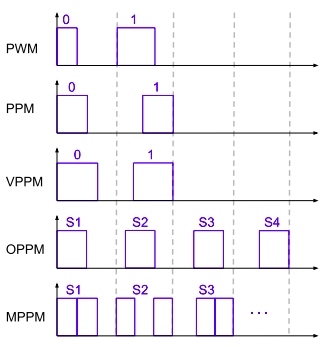
\includegraphics[width=.5\textwidth]{inc/img/ppmvspwm.png}
    \caption{Схематическая диаграмма, показывающая различия между модуляцией длительности импульса (PWM), фазово-амплитудной модуляцией (PPM), переменной фазово-амплитудной модуляцией (VPPM), перекрывающейся фазово-амплитудной модуляцией (OPPM) и многоимпульсной фазово-амплитудной модуляцией (MPPM). $S_n$ обозначает n-ный символ.~\cite{Pathak2015}}
    \label{fig:ppmvspwm}
\end{figure}

\Abbrev{MPPM (multipulse pulse position modulation)}{многоимпульсная фазово-амплитудная модуляция}
В~\cite{Sugiyama1989} была предложена другая схема, основанная на PPM, которая аналогично OPPM даёт возможность передавать несколько импульсов за интервал длительности символа. В отличии от OPPM, однако, здесь импульс не обязательно должен быть непрерывным (смотри рисунок~\ref{fig:ppmvspwm}). Это позволяет повысить спектральную эффективность по сравнению с OPPM~\cite{Shiu1999}.

\Abbrev{VPPM (variable pulse position modulation)}{переменная фазово-амплитудная модуляция}

В самом стандарте, описывающем системы VLC и Li-Fi, IEEE 802.15.7~\cite{IEEE2018} предлагается альтернативная схема модуляции \--- переменная фазово-амплитудная модуляция (VPPM), которая имеет ряд общих черт с PPM и PWM. Как и в первой, данные кодируются фазой импульса, в то время как возможно изменение длительности импульса при необходимости. В результате этого, VPPM имеет высокую надёжность и простоту, и позволяет детально варьировать уровень освещения, как и в PWM~\ref{PWM}.

\subsection{Мультиплексирование с орто­гональным частотным разделением каналов (OFDM)}

Преимущество мультиплексирования с орто­гональным частотным разделением каналов (OFDM), которое широко применяется в РЧ-коммуникациях, является отсутствие межсимвольной интерференции, которая может появляться в описанных выше методах модуляции из-за нелинейности частотного отклика каналов связи. Было предложено использовать OFDM и для систем передачи данных по видимому свету~\cite{Afgani2006}. Особенностью OFDM является то, что канал разделяется на несколько орто­гональных несущих, данные по которым передаются параллельно потоками,  модулируемыми по несущим. Проблема применения OFDM для беспроводных систем связи по видимому свету заключается в том, что OFDM генерирует комплексные биполярные сигналы, которые необходимо сконвертировать в действительные сигналы.

Другой проблемой OFDM является нелинейность отношения приложенного тока к интенсивности света LED~\cite{Burchardt2014}. Это выражается в отношении пиковой к средней мощности и было изучено в~\cite{Elgala2009,Elgala2009}. Там авторы предлагают в качестве решения использование светодиода в небольшом интервале мощности, на котором это отношение квазилинейное. 

Несмотря на эти недостатки, OFDM  имеет высокие перспективы, и было показано, что возможно достижение скорости передачи до нескольких Гб/с с использованием одного светодиода~\cite{Khalid2012,Tsonev2014}.

\subsection{Цветовая манипуляция (CSK)}
\label{CSK}

В стандарте IEEE 802.15.7~\cite{IEEE2018} описывается ещё один тип модуляции, который был разработан специально для использования в беспроводных системах связи по видимому свету \--- цветовая манипуляция (CSK). Суть этого метода заключается в отдельном модулировании трёх цветовых компонент RGB светодиода. 

\begin{figure}[!ht]
    \centering
    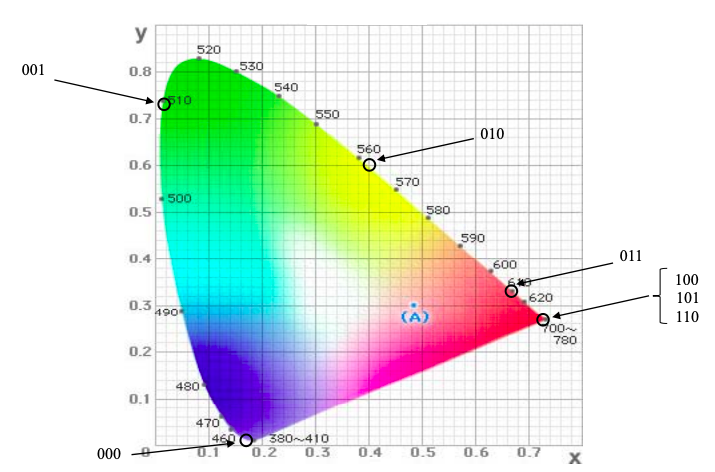
\includegraphics[width=.65\textwidth]{inc/img/cie1931.png}
    \caption{Цветовое пространство CIE 1931~\cite{IEEE2018}}
    \label{fig:cie1931}
\end{figure}

CSK модуляция основана на модели цветового пространства CIE 1931~\cite{CIE1931} (рисунок~\ref{fig:cie1931}, таблица~\ref{table:cie1931}), на которой всем видимым человеческим глазом цветам присвоена пара $(x,y)$ координат. Все это пространство разделено на семь полос, представленных в таблице~\ref{table:cie1931}

\begin{table}[!h]
    \centering
    \begin{tabular}{|c| c| c| c|} 
     \hline
     Полоса (нм) & Код & Центральная длина волны (нм) & $(x,y)$ \\ \hline
     $380-478$ & $(000)$ & $429$ & $(0.169, 0.007)$ \\ \hline
     $478-540$ & $(001)$ & $509$ & $(0.011, 0.733)$ \\ \hline
     $540-588$ & $(010)$ & $564$ & $(0.402, 0.597)$ \\ \hline
     $588-633$ & $(011)$ & $611$ & $(0.669, 0.331)$ \\ \hline
     $633-679$ & $(100)$ & $656$ & $(0.729, 0.271)$ \\ \hline
     $679-726$ & $(101)$ & $703$ & $(0.734, 0.265)$ \\ \hline
     $726-780$ & $(110)$ & $754$ & $(0.734, 0.265)$ \\ \hline
    \end{tabular}
    \caption{Семь полос, используемых в CSK, их коды, центральные длины волн и координаты на цветовом пространстве~\cite{IEEE2018}}
    \label{table:cie1931}
\end{table}

Суть алгоритма кодирования информации заключается в следующем~\cite{IEEE2018}:

\begin{enumerate}
    \item выбираются три точки в цветовом пространстве, которые соответствуют цветам RGB светодиода \--- получается треугольник;
    \item в зависимости от выбранной схемы кодирования (4-CSK, 8-CSK, 16-CSK \--- четыре, восемь и шестнадцать символов, соответственно) определяются координаты символов на плоскости. По сути это является задачей на оптимизацию, так как необходимо выбрать координаты так, чтобы расстояние между ними было наибольшим (это необходимо для минимизации интерференции между символами);
    \item по координатам символов вычисляется яркость компонент RGB светодиода:
    \begin{equation}
        \begin{gathered}
            x_s = P_i x_i + P_j x_j + P_k x_k \\
            y_s = P_i y_i + P_j y_j + P_k y_k \\
            P_i + P_j + P_k = 1
        \end{gathered}
    \end{equation}

    Здесь $(P_i, P_j, P_k)$ \--- яркости компонент светодиода, $(x_s, y_s)$ \--- цветовые координаты символа на цветовой плоскости (рисунок~\ref{fig:cie1931}), $(x_{ijk}, y_{ijk})$ \--- координаты центральных длин волн компонент светодиода на цветовой плоскости. 
\end{enumerate}

Для большего уменьшения межсимвольной интерференции возможно использовать светодиоды с четырьмя цветовыми компонентами (циан, синий, желтый, красный), так как тогда форма области на цветовой диаграмме будет четырёхугольником (а не треугольником, как в случае RGB светодиода), что позволит расположить символы дальше друг от друга~\cite{Singh2014}.



  \backmatter %% Здесь заканчивается нумерованная часть документа и начинаются ссылки и

  % \include{50-conclusion} %% заключение


  %
% Список литературы при помощи BibTeX
%

% Книги без цитирования, которые будут отображаться в конце списка
% \nocite{kotlinInAction, cleanCode, gofPatterns, koldayev, gitProfessional, rxJava}

\bibliographystyle{ugost2008}
\bibliography{main}



  \appendix % Тут идут приложения

%   \include{70-appendix1}

\end{document}
